\section{Kitaev Triangle}

\begin{figure}[!ht]
  \hspace{-18pt}
  \subfloat[]{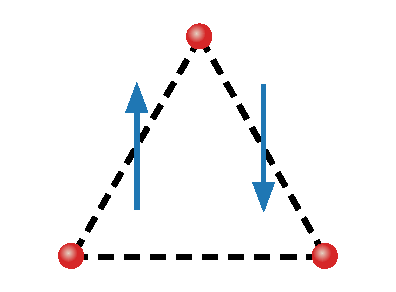
\includegraphics[width=3.0 in]{./figures/3-point-triangle.pdf}}
  \subfloat[]{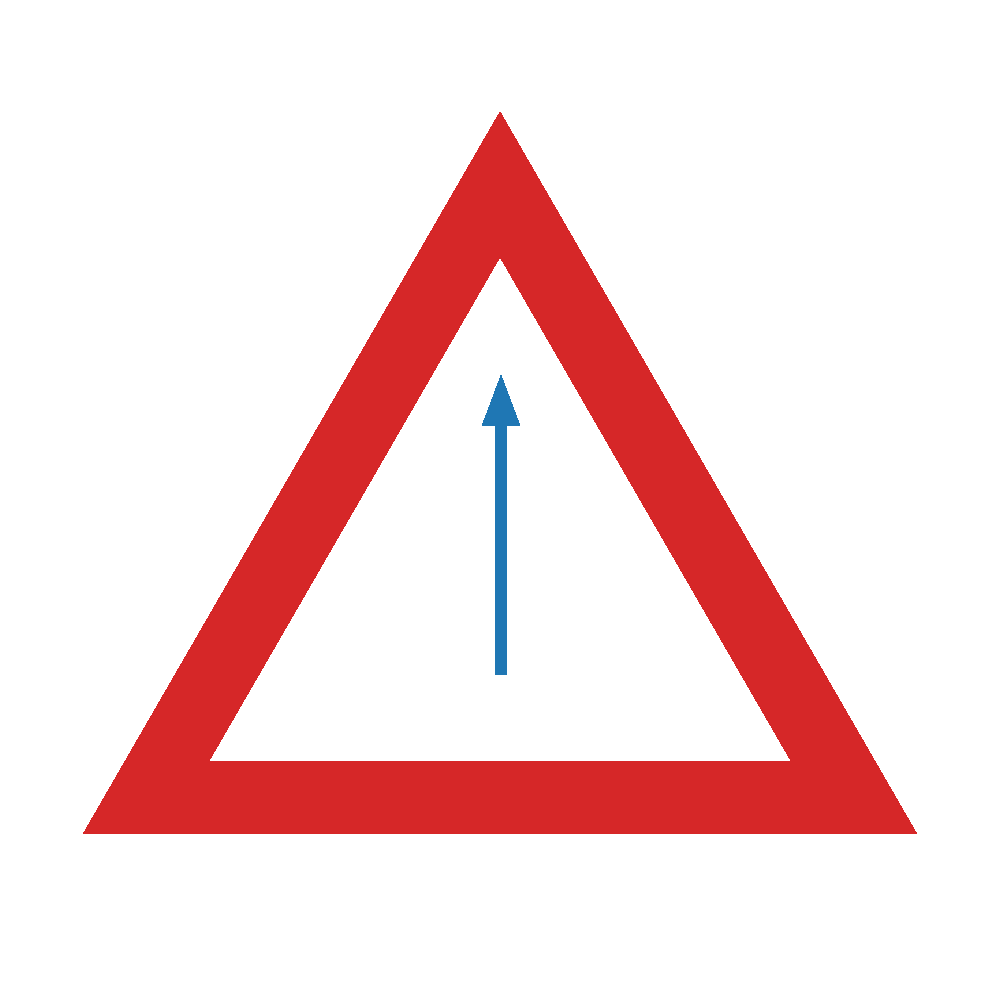
\includegraphics[width=2.4 in]{./figures/hollow-triangle-constant-vector-potential.pdf}}
  \caption{Schematics of two triangle structures proposed in this work. (a) Three-site Kitaev triangle with bond-dependent Peierls phases. (b) Hollow triangular island with a uniform vector potential.}
  \label{fig:triangles}
\end{figure}


In this section we present an exactly solvable minimal model with three sites forming a ``Kitaev triangle" that can host MZM at different pairs of vertices controlled by Peierls phases on the edges. The Bogoliubov-de Gennes (BdG) Hamiltonian includes complex hopping and $p$-wave pairing between three spinless fermions forming an equilateral triangle [Fig.~\ref{fig:triangles} (a)]:
\begin{equation}\label{eq:HBdG}
  \ham = \sum_{\langle j l \rangle} (-te^{i\phi_{jl}}\cc_{j} c_l + \de e^{i\theta_{jl}} c_{j} c_l + {\rm h.c.}) - \sum_{j} \mu \cc_j c_j,
\end{equation}
where $t$ is the hopping amplitude, $\de$ is the amplitude of the (2D) $p$-wave pairing, $\mu$ is the chemical potential, $\theta_{jl}$ is the polar angle of $\mathbf r_{jl} = \mathbf r_l - \mathbf r_j$ (the $x$ axis is chosen to be along $\mathbf r_{12}$), consistent with $\{c^\dag_l, c^\dag_j\} = 0$. $\phi_{jl}$ is the Peierls phase due to a bond-dependent vector potential $\mathbf A$ to be specified below (the nearest neighbor distance $a$ is chosen to be the length unit hereinbelow):
\begin{eqnarray}
\phi_{jl} = \dfrac{e}{\hbar} \int_{\mathbf r_j}^{\mathbf r_{l}} \vec{A} \cdot d\vec{l} = -\phi_{lj}
\end{eqnarray}
where $e>0$ is the absolute value of the electron charge. Below we use the natural units $e=\hbar=1$. To get the conditions for having MZM in this model we rewrite $\mathcal{H}$ in the Majorana fermion basis $a_{j} = c_j + c^\dag_j$, $b_j = \frac{1}{i}(c_j - c^\dag_j)$:
\begin{align}\label{eq:H3M}
    \ham =  -\dfrac{i}{2} \sum_{\langle j l \rangle} \Big[&\left(t\sin\phi_{jl}-\de\sin\theta_{jl}\right) a_j a_l \\\nonumber
  +&\left(t\sin\phi_{jl}+\de\sin\theta_{jl}\right) b_j b_l  \\\nonumber
  +&\left(t\cos\phi_{jl} - \de\cos\theta_{jl}\right) a_j b_l  \\\nonumber
  -&\left(t\cos\phi_{jl}+\de\cos\theta_{jl}\right) b_j a_l\Big]  -\dfrac{i\mu}{2} \sum_j  a_j b_j
\end{align}
For concreteness we consider the Kitaev limit $t=\de$, $\mu=0$, and choose $\phi_{12} = 0$ so that sites 1 and 2 alone form a minimal Kitaev chain with $\mathcal{H}_{12} = itb_1a_2$ and hosting MZM $a_1$ and $b_2$. In order for the MZM to persist in the presence of site 3, one can choose $\phi_{23}$ and $\phi_{31}$ so that all terms involving these Majorana operators cancel out. For example, consider the $2-3$ bond, for which $\theta_{23} = 2\pi/3$, we require
\begin{eqnarray}
    \sin\phi_{23} + \sin\frac{2\pi}{3} =\cos\phi_{23} + \cos\frac{2\pi}{3} = 0
\end{eqnarray}
which means $\phi_{23} = -\pi/3$. Similarly one can find $\phi_{31} =-\phi_{13} = -\pi/3$. The three Peierls phases can be realized by the following staggered vector potential
\begin{equation}\label{eq:Astep}
  \vec{A} =\left[1-2\Theta(x)\right]\frac{2 \pi}{3\sqrt{3}} \hat{y}
\end{equation}
where $\Theta(x)$ is the Heavisde step function. In fact, using a uniform $\vec{A} =\frac{2 \pi}{3\sqrt{3}} \hat{y}$, which corresponds to $\phi_{23} = -\pi/3 = -\phi_{31}$ also works, since the existence of $a_1$ is unaffected by $\phi_{23}$. However, in this case the counterpart of $b_2$ is not localized on a single site. For the same reason, the above condition for MZM localized at triangle corners can be generalized to Kitaev chains forming a triangular loop, as well as to finite-size triangles of 2D spinless $p$-wave superconductors in the Kitaev limit, as the existence of $a_1$ and $b_2$ are only dictated by the vector potential near the corresponding corners. It should be noted that in the latter case, 1D Majorana edge states will arise when the triangle becomes larger, and effectively diminish the gap that protects the corner MZM.  On the other hand, for the longer Kitaev chain, due to the potential practical difficulty of controlling further-neighbor hopping and pairing amplitudes, it is better to resort to the approach of controlling the individual topological phases of the three edges which will be detailed in the next section.

We next show that the minimal Kitaev triangle suffices to demonstrate braiding of MZM. To this end we consider a closed parameter path linearly interpolating between the following sets of values of $\phi_{jl}$:
\begin{eqnarray}
    (\phi_{12},\phi_{23},\phi_{31}) &=& \left(0,-\frac{\pi}{3},-\frac{\pi}{3}\right ) \equiv \bm \phi_1 \\\nonumber
    &\rightarrow& \left(-\frac{\pi}{3},-\frac{\pi}{3},0 \right) \equiv \bm \phi_2 \\\nonumber
    &\rightarrow& \left(-\frac{\pi}{3},0,-\frac{\pi}{3} \right) \equiv \bm \phi_3 \\\nonumber
    &\rightarrow& \bm \phi_1
\end{eqnarray}
It is straightforward to show that at $\bm \phi_{2}$ and $\bm \phi_3$ there are MZM located at sites $3,1$ and $2,3$, respectively. Therefore the two original MZM at sites $1,2$ should switch their positions at the end of the adiabatic evolution.

\begin{figure}[!ht]
	\centering
  \hspace{-27pt}
  \subfloat[]{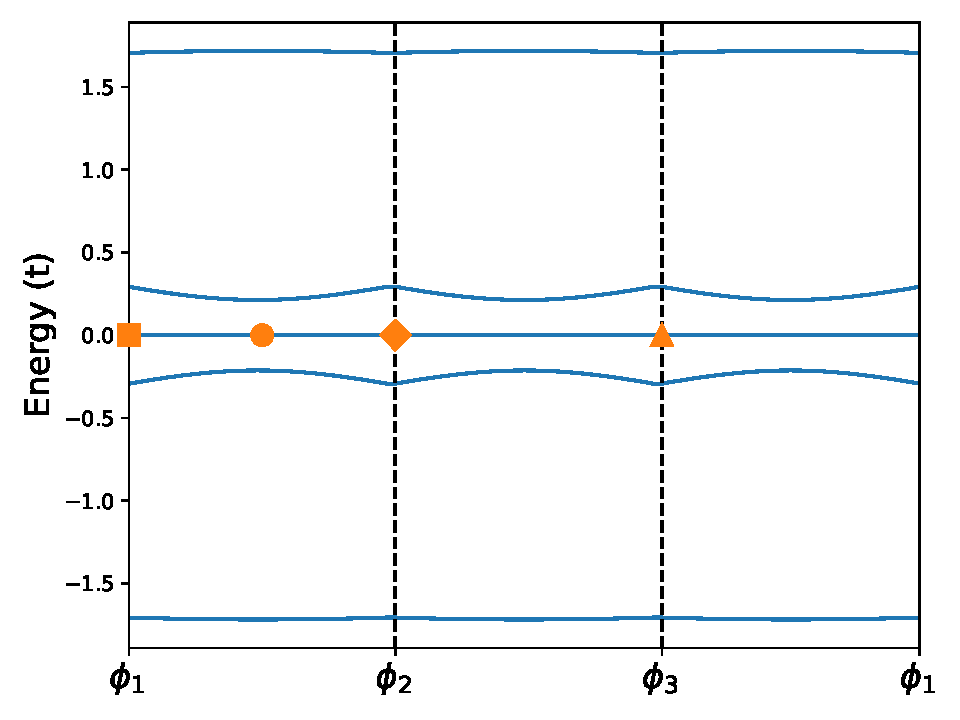
\includegraphics[width=3.3 in]{./figures/3eigval.pdf}}\\
  \subfloat[]{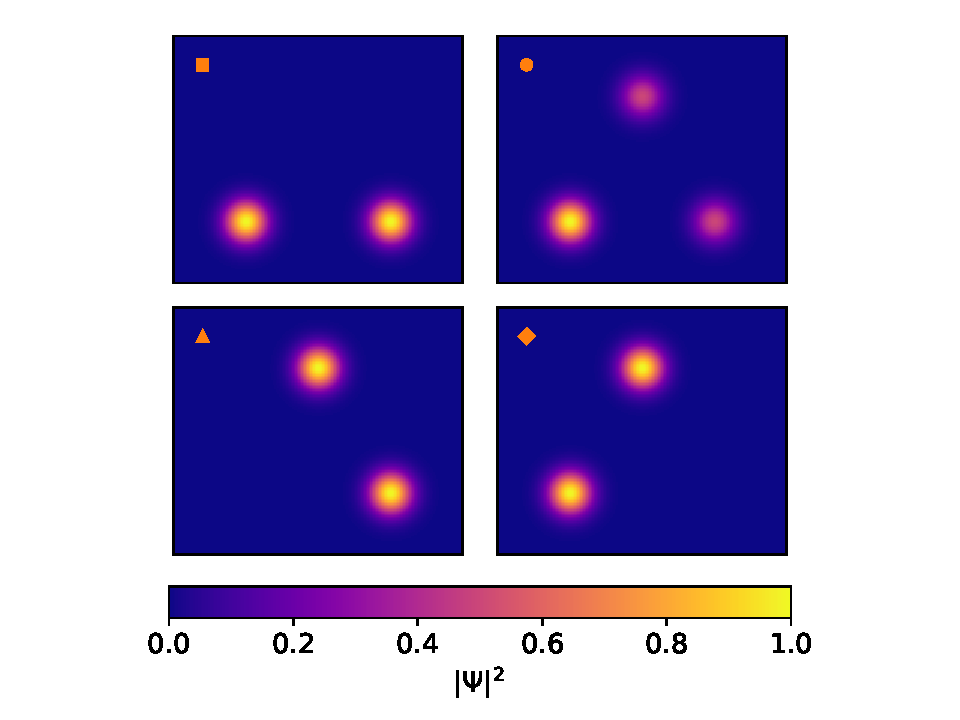
\includegraphics[width=4.2 in]{./figures/3eigvec.pdf}}
	\caption{(a) Evolution of the eigenvalues of the 3-site Kitaev triangle along the closed parameter path for $\phi$ on the three edges. (b) MZM wavefunctions at different points of the parameter path. Clockwise from the upper left panel: $\bm \phi_1 \rightarrow \frac{1}{2}(\bm \phi_1 + \bm \phi_2)\rightarrow \bm \phi_2\rightarrow \bm \phi_3$.}
	\label{fig:3eig}
\end{figure}

Indeed, Fig.~\ref{fig:3eig} shows that the MZM stays at zero energy throughout the parameter path that interchanges their positions. To show that such an operation indeed realizes braiding, we explicitly calculated the many-body Berry phase of the evolution \cite{supp,aliceaNonAbelianStatisticsTopological2011,liManipulatingMajoranaZero2016} and found the two degenerate many-body ground states acquire a $\frac{\pi}{2}$ difference in their Berry phases as expected \cite{aliceaNonAbelianStatisticsTopological2011}. Compared to the minimum T-junction model with four sites \cite{aliceaNonAbelianStatisticsTopological2011}, our Kitaev triangle model only requires three sites to achieve braiding between two MZM, and is potentially also easier to engineer experimentally. In the next section we will show that a more mesoscopic hollow-triangle structure can achieve similar results and may be preferred in other materials platforms.

